\documentclass[11pt, spanish]{article}
\usepackage[spanish, activeacute]{babel}
\usepackage[utf8]{inputenc}
\usepackage{graphicx}
\usepackage{algorithm}
\usepackage{algorithmic}
\usepackage{fullpage}
\renewcommand{\baselinestretch}{1.3}
\floatname{algorithm}{Algoritmo}

\begin{document}
\title{Introducción a la Programación Multinúcleo\\Evolución genética de imágenes}
\author{Daniel Barreto - \#04-36723 \texttt{<daniel@gia.usb.ve>} \\ Ernesto Level - \#05-38402 \texttt{<ealevel@gmail.com>}}
\date{\today}

\maketitle

\section{Introducción}
\subsection{Evolucionando imágenes}
\begin{figure}[htp]
	\centering
	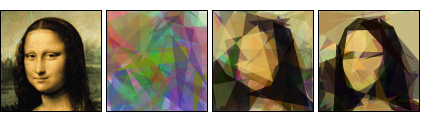
\includegraphics[scale=0.7]{media/evolution.png}
\end{figure}

Conseguir la mejor aproximación a una imagen dada usando una cantidad finita de polígonos.

\subsection{Características de la evolución}
\begin{itemize}
	\item Se busca representar lo mejor posible una imagen dada con un número finito y estático de polígonos (104 en nuestro caso de estudio)
	\item Cada polígono tiene una cantidad estática de vertices (6 en nuestro caso de estudio), un color y una opacidad.
	\item Se utilizan individuos cuyos \emph{ADN} representan una secuencia del número de polígonos a utilizar, guardando el color de relleno del polígono, la opacidad con la que es dibujado en pantalla y sus vertices.
\end{itemize}

\section{Marco teórico}
\subsection{Aproximaciones a la solución}
Existen dos aproximaciones estudiadas para lograr una evolución de la imagen:

\begin{enumerate}
	\item \textbf{Roger Alsing:} Utiliza una población de sólo un individuo, que representa una cantidad de polígonos variable, empieza con un único polígono y luego va agregando mas. Realiza mutaciones con poca probabilidad para ir variando las posiciones y los colores de los polígonos que representa el individuo. Parecido a \emph{Hill Climbing}
	\item \textbf{Jacob Seidelin:} Utiliza una población variable, pero de más de un individuo. Los individuos con mejor fitness se cruzan y se generan nuevas poblaciones. Aproximación netamente genética.
	\end{enumerate}

\subsection{Estructuras de datos y representaciones}

\section{Implementación}
Para la resolución de este problema se utilizó un algoritmo genético, éste partia de la creación de una población de individuos generados aleatoriamente. \\

A partir de esta población se genera una nueva, esto se hace tomando los mejores individuos para cruzarlos y mutarlos. Esta nueva población generada toma el lugar de la población anterior, y en caso que el mejor individuo de esa población sea el mejor individuo encontrado hasta el momento, se dibuja. Este último de paso se hace un número $n$ de veces, mientras más veces se realice mejores individuos se van consiguiendo y mejor la solución generada se parece a la imagen original. \\

\subsection{Descripción del algorítmo usado}
A continuación se presenta la base del algoritmo utilizado para la resolución del problema, considerando una población de 36 individuos, donde cada unos de ellos posee 48 polinomios, y a su vez cada uno de ellos posee un alfa y colores (RGB por rojo, verde y azul), y dos coordenadas $X$ e $Y$ por cada uno de los 6 vertices con los que se trabaje. \\

El algoritmo \ref{genetic} muestra el algoritmo genético utilizado para la resolver el problema.

\begin{algorithm}
	\caption{Algoritmo Genético}
	\label{genetic}
	\begin{algorithmic}
		\STATE Crear una población inicial con individuos generados aleatoriamente.
		\FOR {$i$ \textbf{in} $1..n$}
			\STATE Generar una nueva población a partir de la población anterior.
			\STATE Reemplazar la población actual con la nueva población.
			\IF {El mejor individuo de la población actual es el mejor individuo}
				\STATE Dibujar mejor individuo de la población actual.
			\ENDIF
		\ENDFOR
	\end{algorithmic}
\end{algorithm}

\subsection{Patrones de selección}
Para la generación de la nueva población se decidió tomar los mejores 6 individuos de la población como el primer padre, y por cada uno tomar 6 otros individuos escogidos aleatoriamente y cruzarlos, dando como resultado una población de 36 individuos.

\subsection{Cruce de individuos}
El nuevo individuo a crear será una mezcla de los polígonos que conforman los \emph{ADN} de ambos padres, elegidos uniformemente aleatorios. Esto se hace con un factor de probabilidad del 50\% entre tomar el cromosoma del primer padre o tomar el del segundo padre.

\subsection{Mutación del individuo}
El nuevo individuo generado pasa un proceso de mutación, en donde con una probabilidad del 2\% se decide si se muta uno de los cromosomas del individuo o no, esto se hace para todos sus cromosomas. \\

En caso que se desee mutar el cromosoma, se tomará el cromosoma y podrá mutar hasta un 10\%; esto significa que su valor podrá variar hasta un máximo de 10\% por encima o debajo de su valor. Así:
$$ cromosoma = cromosoma + random * 10\% * 2 - 10\% $$

Considerando que el \emph{random} genera número entre 0 y 1, se tiene que el máximo número resultante sería $cromosoma + 0,1$ y el mínimo $cromosoma - 0,1$.

\subsection{Función de Fitness}
La función de fitness utilizada simplemente calcula pixel a pixel la diferencia de colores entre la imagen original y la imagen generada; esto permite distinguir a todos los individuos generados y tomar el mejor, es decir, quien tenga mayor fitness.

$$ F_{fitness} = \displaystyle\sum_{pixel} \delta_r + \delta_g + \delta_b $$

donde $\delta_i$ indica la diferencia absoluta entre el pixel de la imagen original y la imagen generada, para $i = \{r, g, b\}$ indicando respectivamente los colores: rojo, verde y azul.

\section{Paralelización}
\subsection{SPU}
El cómputo más fuerte se realiza en el cálculo del fitness de un individuo. Sin embargo, el SPU no poseía las librerías necesarias para realizar esto, y aunque se buscó y trató de compilar los archivos fuentes de la librería necesario no nos fue posible la paralelización de esta función. \\

Sin embargo, se paralelizó el calculo de los nuevos individuos. Como una población de individuos es de tamaño 36, tomando 6 primeros padres y otros 6, se decidió paralelizar esta generación generando uno de cada 6 individuos por ver a cada SPU. \\

Es decir, al tomar el primer padre y se debían generar 6 otros padres aleatorios, el calculo del cruce de estos padres lo hacían los SPU. Y se repetía para los siguientes cinco primeros padres restantes.

\subsection{PPU}
El \emph{PPU} se encarga de llevar el manejo principal de la ejecución. Se encarga de distribuir la carga entre los SPU, luego de cada generación se encarga del cálculo del fitness, al tener la población se encarga de tomar el mejor individuo y dibujarlo. \\

El peso en memoria de un individuo viene dado principalmente por el peso del \emph{ADN} que representa, el cual puede ser estáticamente calculado de la siguiente forma:

$$ Peso_{poligono} = Peso_{colores} + Peso_{vertices} = 4 + 2*6 = 16\textrm{ floats} $$

$$ Peso_{ADN} = NUM\_POLIGONOS * Peso_{poligono} = 48 * 16 = 768\textrm{ floats} $$

El peso de un color ocupa 4 bytes (rojo, verde, azul, alfa). El peso de un vértice pesa 12, ya que se utilizan 6 vértices, donde cada uno indica las coordenadas X e Y del punto.

\subsection{Posible \emph{Loop Unrolling}}
\textbf{Cálculo de fitness} contiene dos ciclos anidados que iteran 128 veces cada uno (por el tamaño de la imagen: 128x128 pixeles), siendo el total de iteraciones $128 * 128 = 16384$. \\

Aprovechando las operaciones \emph{Vector/SIMD} se redujo el total de iteraciones a $128 * (128/4) = 4096$. Logrando reducir hasta un \textbf{75\%} el número de iteraciones.

\section{Resutados}
\end{document}
